% !TEX root = ../../../main/aws_chabauty.tex
\newpage
\subsection{Lecture 2}

$\int$'s are locally analytic.

$P \in X(\F_p)$, $Q_1,Q_2 \in [P] \ma{\sim} P \hat{i} P$, given by $Q \mapsto t(Q)$, $t$ with respect to $P$.
	\[
	\int_{Q_1}^{Q_2} \omega= \int_{t_1}^{t_2} f(t) \;dt= \sum \dfrac{d_i t^{i+1}}{i+1} \bigg|_{t_1}^{t_2}= I_i(t)
	\]
by the Fundamental Theorem of Calculus.
	\[
	\omega \bigg|_{[P]}= f(t) \;dt= \sum a_i t^i, \quad a_i \in \Z_p
	\]


\begin{thm}[Coleman]
If $X/\Q$ is nice, $r<g$, and $p$ is a good prime with $p> 2g$, then $\#X(\Q) \leq \#X(\F_p) + 2g-2$.
\end{thm}


\pf Let $Q \in X(\F_p)$ and let $\omega \in V$ be a fixed annihilating differential. Let $n_\Q= \deg(\div \omega \cap [Q])$, then $\#\{z \in p \Z_p \colon I_i(z)=0 \} \leq 1+ n_\Q$. Then $\#X(\Q) \leq \#X(\Qp)_1$ (the $\Qp$ solutions to these integrals, i.e. the $\Qp$ points that vanish under the abelian integral). But this is at most $\sum_{Q \in X(\F_p)} (1+ n_\Q)$


	\begin{figure}[!ht]
	\centering
	\includegraphics[width=0.4\textwidth]{../images/im6.png}
	\end{figure}


But then we have
	\[
	\begin{aligned}
	\#X(\Q) &\leq \#X(\Qp)_1 \\
	&\leq \sum_{Q \in X(\F_p)} (1+ n_\Q) \\
	&= \sum_{\alpha \in X(\F_p)} + \sum_{\alpha \in X(\F_p)} n_\Q \\
	&\leq \#X(\F_p) + \underbrace{2g-2}_{\deg \omega} 
	\end{aligned}
	\]
\qed \\


\begin{rem}
We did not really compute an upper bound on $\#X(\Q)$, but rather $\#X(\Qp)_1$, which is strictly larger. 
\end{rem}


\begin{lem}[Coleman]
Let $f(t)= \sum \dfrac{a_i}{i+1} \in \Qp[i+1]$ such that $f'(t)= \sum a_i t^i \in \Z_p[i+1]$. Let $m= \ord_{t=0} (f'(t) \mod p)$.\footnote{Note, $m=n_\Q$)} Suppose that $m < p-2$.\footnote{By the previous footnote, $p>m+2$ implies that $m \leq 2g-2$ by Riemann-Roch.} Then $f$ has at most $m+1$ zeros in $p \Z_p$. 
\end{lem}

\pf Newton polygons.

	\begin{figure}[!ht]
	\centering
	\includegraphics[width=0.5\textwidth]{../images/im7.png}
	\end{figure}
	

Note that $v(a_m)=0$. Because of the bound on $p$. Then $v(m+1)=0$. Then $v(a_i)>0$ for $i<m$ and $v(i+1)=0$ for $i<m$. But
	\[
	v\left( \dfrac{a_i}{i+1} \right) \geq v_p(i+1) > m+1 - (i+1)
	\]
Segments of slope $\alpha$ correspond to roots with valuation $-\alpha$. The length of the segment corresponds to the number of roots. \qed \\


If $X/\Qp$ is any variety, then $\trep X:= \ov{v(X(\ov{\Qp}))}$. 


\begin{ex}
$x+y= 1$, then
	
	\begin{figure}[!ht]
	\centering
	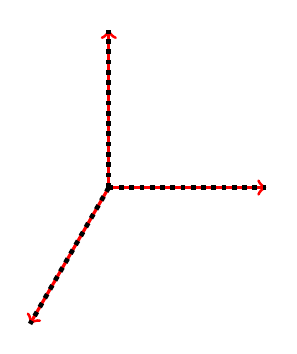
\begin{tikzpicture}
	
	\draw[line width=0.04cm,->,red] (0,0) -- (2,0);
	\draw[line width=0.04cm,->,red] (0,0) -- (0,2);
	\draw[line width=0.04cm,->,red] (0,0) -- (-1,-1.732);
	
	\draw[line width=0.06cm,dotted] (0,0) -- (2,0);
	\draw[line width=0.06cm,dotted] (0,0) -- (0,2);
	\draw[line width=0.06cm,dotted] (0,0) -- (-1,-1.732);
	
	\end{tikzpicture}
	\end{figure}
\end{ex}


\begin{ex}
$xyz= p(x^3+y^3+z^3)$
	\begin{figure}[!ht]
	\centering
	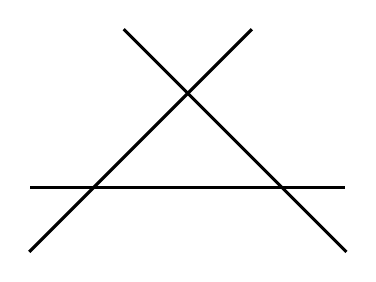
\begin{tikzpicture}[scale=2]
	\draw[line width=0.04cm] (-1,-0.3) -- (1,-0.3);
	\draw[line width=0.04cm] (-1.007,-0.707) -- (0.407,0.707);
	\draw[line width=0.04cm] (-0.407,0.707) -- (1.007,-0.707);
	\end{tikzpicture}
	\end{figure}

	\begin{figure}[!ht]
	\centering
	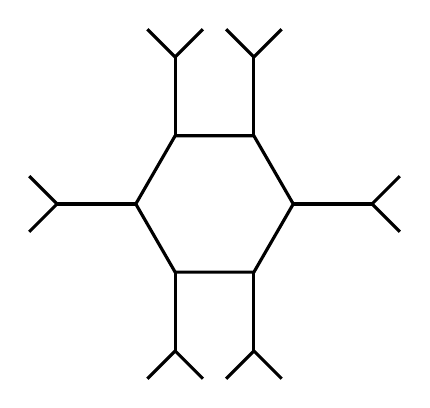
\begin{tikzpicture}[scale=1]
	\draw[line width=0.04cm] (1,0) -- (0.5,0.866) -- (-0.5,0.866) -- (-1,0) -- (-0.5,-0.866) -- (0.5,-0.866) -- (1,0);
	\draw[line width=0.04cm] (1,0) -- (2,0); 
		\draw[line width=0.04cm] (2,0) -- (2.353,0.353);
		\draw[line width=0.04cm] (2,0) -- (2.353,-0.353);
	\draw[line width=0.04cm] (0.5,0.866) -- (0.5,1.866);
		\draw[line width=0.04cm] (0.5,1.866) -- (0.853,2.219);
		\draw[line width=0.04cm] (0.5,1.866) -- (0.147,2.219);
	\draw[line width=0.04cm] (-0.5,0.866) -- (-0.5,1.866);
		\draw[line width=0.04cm] (-0.5,1.866) -- (-0.147,2.219);
		\draw[line width=0.04cm] (-0.5,1.866) -- (-0.853,2.219);
	\draw[line width=0.04cm] (-1,0) -- (-2,0);
		\draw[line width=0.04cm] (-2,0) -- (-2.353,0.353);
		\draw[line width=0.04cm] (-2,0) -- (-2.353,-0.353);
	\draw[line width=0.04cm] (-0.5,-0.866) -- (-0.5,-1.866);
	 	\draw[line width=0.04cm] (-0.5,-1.866) -- (-0.147,-2.219);
		\draw[line width=0.04cm] (-0.5,-1.866) -- (-0.853,-2.219);
	\draw[line width=0.04cm] (0.5,-0.866) -- (0.5,-1.866);
		\draw[line width=0.04cm] (0.5,-1.866) -- (0.853,-2.219);
		\draw[line width=0.04cm] (0.5,-1.866) -- (0.147,-2.219);
	\end{tikzpicture}
	\end{figure}
\end{ex}



% Stoll's Idea
\subsubsection{Stoll's Idea}

Choose the `best' $\omega$ for each $Q \in X(\F_p)$. Let $n_Q(\omega)= \deg(\div w(J \otimes L))$, $n_Q= \min_{W \in V} n_Q(\omega)$. 
	\[
	\#X(\Q) \leq \sum_{Q \in X(\F_p)} (1 + n_Q) \leq \#X(\F_p) + \sum_{Q \in X(\F_p)} n_Q
	\]
Now define $D:= \sum_{Q \in X(\F_p)} n_q[Q]$. We claim that $\deg D \leq 2r$. Now $\dim V \geq g-r$. Observe that $D$ is special. If $K_D$ is a canonical divisor, then $D$ is special if $\dim H^0(X,K \setminus D) \geq 1$. Then there exists same canonical divisor $K^1 \geq 0$ such that $D \leq K^1$. Now $\dim H^0(X,\Omega^1(-D)) >0$ containing $\omega$ if and only if $\div \omega \geq D$. 


\begin{thm}[Clifford]
If $D$ is special, then $\dim H^0(X,D) \leq \dfrac{\deg D}{\alpha} + 1$. 
\end{thm}


Context (Riemann-Roch). $h^0(D) - h^0(K-D)= \deg D+1-g$.

\pf $D= \sum n_q [Q]$.
	\[
	V \subseteq H^0(X_{\F_p}, \Omega^1(-D))
	\]
Then $g-r \leq \dim H^0(\Omega^1(-D)) \leq \frac{1}{2} (2g-2 - \deg D)+1$. But then $\deg D \leq 2r$. \qed \\


The notion of special is not good for singular curves. $H^0(D) \in P$. $K$ is not often special, there exist curves such that there does not exist an effective canonical divisor. 


	\begin{figure}[!ht]
	\centering
	\includegraphics[width=0.5\textwidth]{../images/im11.png}
	\end{figure}



















